\chapter{Realisierung} \label{ch:results}

Dieses Kapitel befasst sich mit der Realisierung dieses Projekts und die Ereignisse, die währenddessen entstanden sind.


Vor der Realisierung des Projekts ist auch wichtig zu wissen, wie die Daten in dem Staging Bereich des \ac{dw} des \ac{diz} an der Universitätsmedizin Mainz gespeichert werden, und wie diese Daten danach im \ac{diz} bearbeitet werden (\ref{fig:dizummz}).

\begin{figure}[ht]
	\centering
	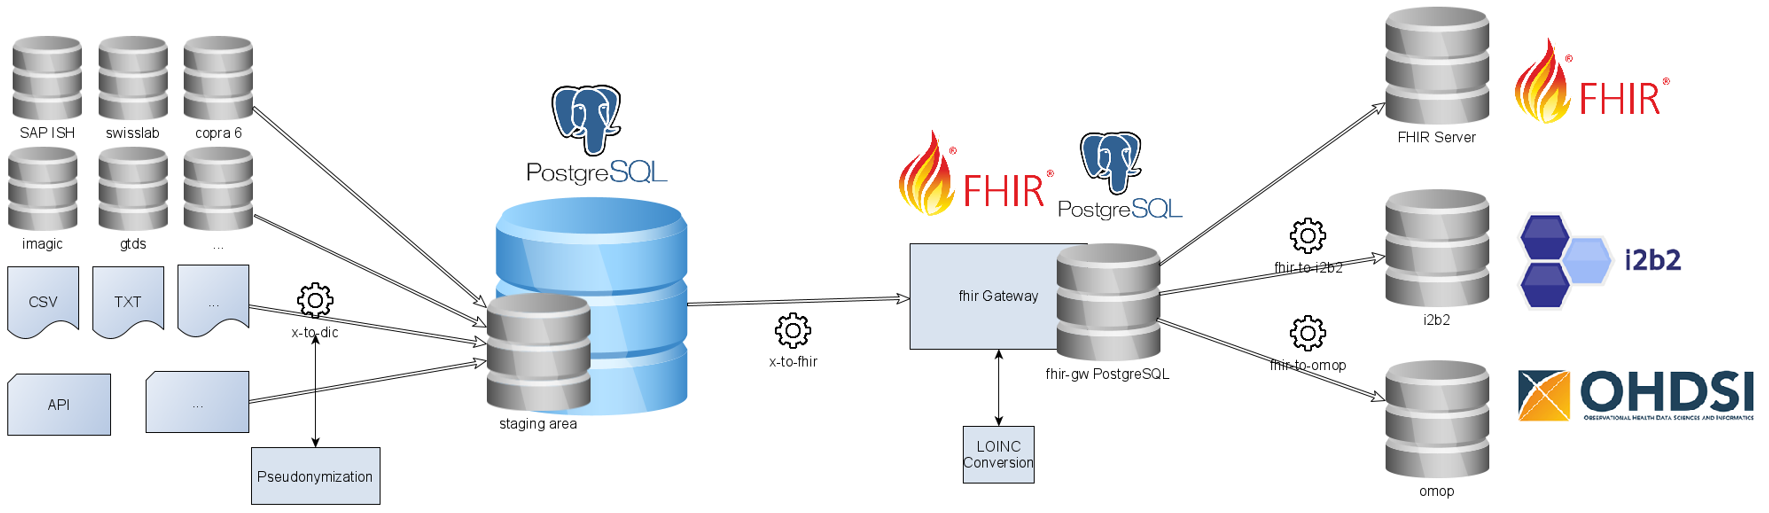
\includegraphics[height=4cm]{figures/diz_ummz}
	\caption[\acs{diz}-Struktur an der Universitätsmedizin Mainz] {\acs{diz}-Struktur an der Universitätsmedizin Mainz. Die Daten aus den verschiedenen Quellen in der Klinik werden pseudonymisiert in dem Staging Bereich des \ac{dw} gespeichert. Diese Daten werden danach bearbeitet und in \ac{fhir} überführt. Am Ende wird die aggregierte Information in Werkzeuge wie i2b2 oder OMOP präsentiert.}
	\label{fig:dizummz}
\end{figure}

Für die Realisierung dieses Projekts wurde mit der Information der \ac{copra}-Instanz des Staging Bereichs des \ac{dw} gearbeitet (\ref{fig:components}).

 Zu Beginn wurde die \ac{db} \texttt{mii\_copra} entwickelt. In den Tabellen dieser \ac{db} wurden die Parameter der \ac{fhir}-Profile des Erweiterungsmodul \glqq Intensivmedizin\grqq{} zusammen mit den relevanten Konfigurationsvariablen von \ac{copra} aus der \ac{copra}-Instanz des Staging Bereichs des \ac{dw} des \ac{diz} importiert. In der \ac{db} \texttt{mii\_copra} wurden auch die Zwischenschritten des Data Mappings realisiert. Als Ergebnis dieses Prozesses wird ein Datensatz mit zugeordneten Konfigurationsvariablen mit \ac{fhir}-Profilen erzeugt. Dieser Datensatz wurde danach in der \ac{copra}-Instanz des Staging Bereichs des \ac{dw} importiert. Mit diesem Datensatz als Basis wurden \ac{sql}-Views für die Zusammenführung der Daten beider Systeme programmiert.

Ein Diagramm mit den Komponenten und dem Fluss der Daten in diesem Projekt ist in der \ref{fig:components} dargestellt.
%\clearpage

\begin{figure}[ht]
	\centering
	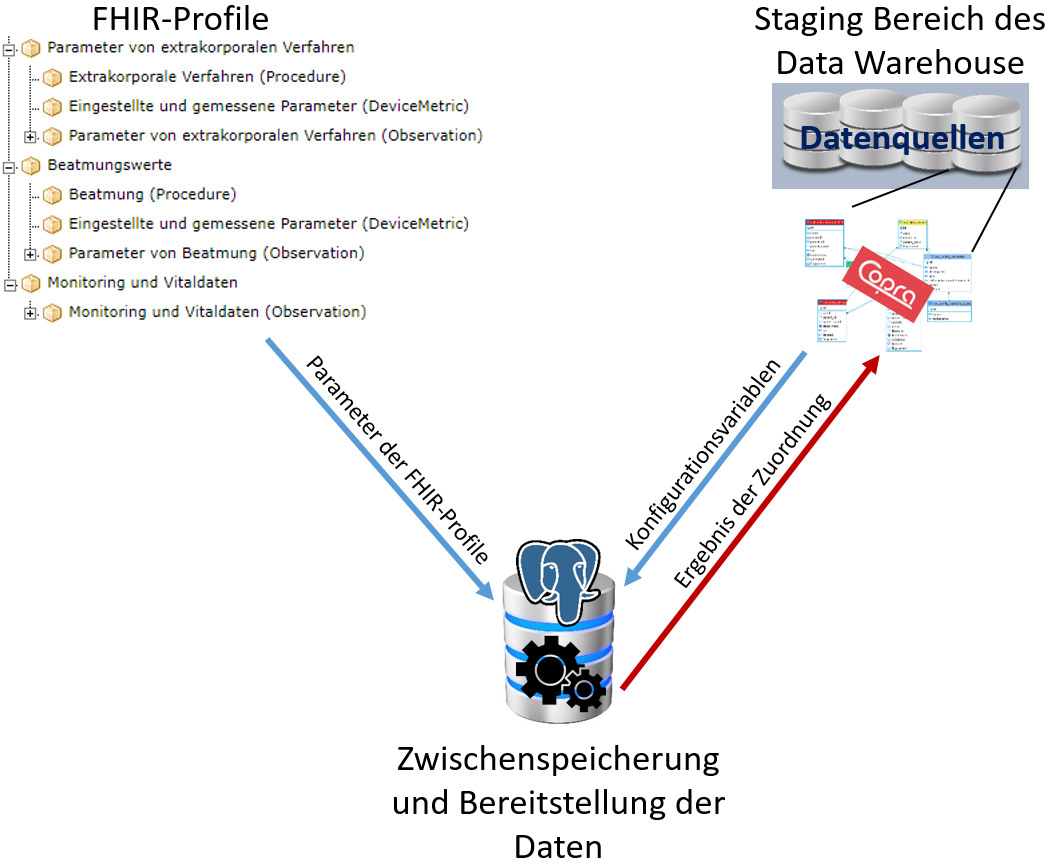
\includegraphics[height=9.5cm]{figures/master_diagram}
	\caption[Komponenten und Fluss der Daten] {Komponenten und Fluss der Daten in diesem Projekt.}
	\label{fig:components}
\end{figure}